\chapter{Introduction}
\section{Motivation}
{\Large
 \begin{itemize}
  \item Small vertical beam size ({\color{red} goal 1})
  \begin{itemize}
   \item Achieve $\sim 37$nm
   \item Validate Local chromaticity correction
  \end{itemize}
  \item Stabilization of beam center ({\color{blue} goal 2})
  \begin{itemize}
   \item down to $\sim2$nm
  \end{itemize}
 \end{itemize}
}
 $\,$
  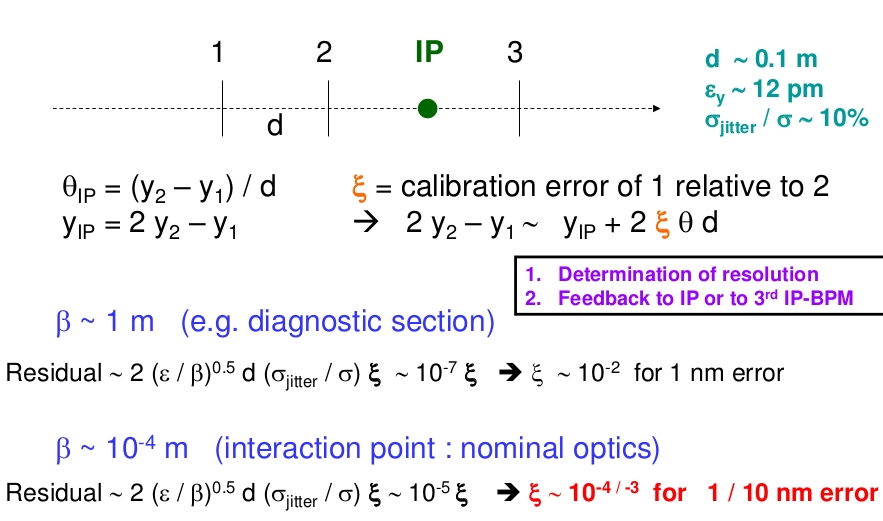
\includegraphics[angle=0,scale=0.35]{scalefactors.jpg}
{\LARGE
  \begin{itemize}
   \item Locate BPMs to enable the \textbf{ maximum possible} beam position resolution
   \item Precision $\sim 5\mu$m
   \item Calibration $\sim 10^{-4}$
  \end{itemize}
 \hspace*{5cm}$\Downarrow$\\
 Displace each BPM block \textbf{independently}
 }\par
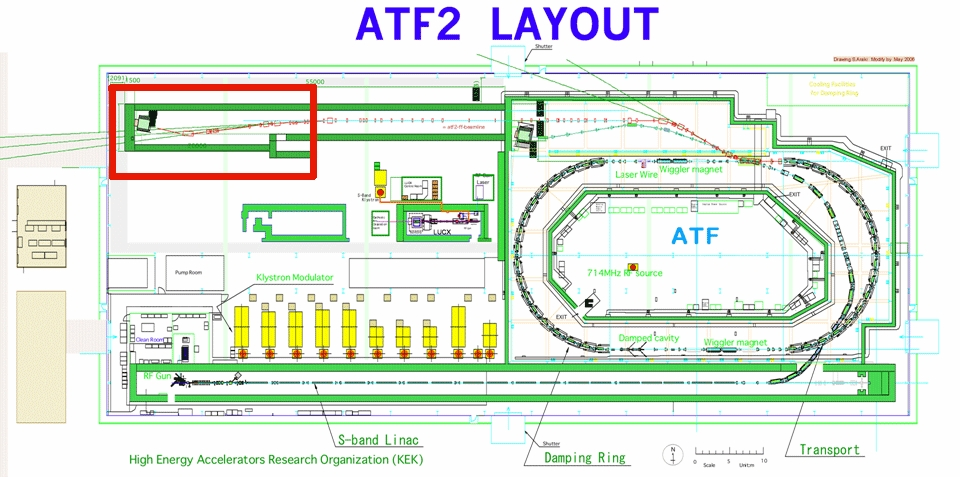
\includegraphics[angle=0,scale=0.2]{ATF2layout33.jpg}
% \end{frame}
% \begin{frame}
\hspace{1cm}
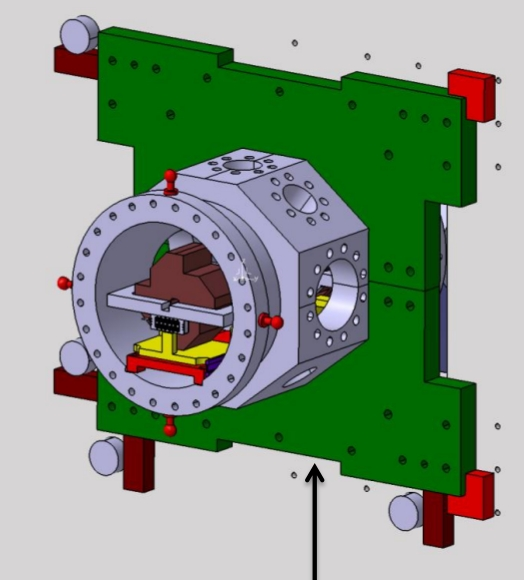
\includegraphics[angle=0,scale=0.16]{chambrevide.jpg}\\
\hspace*{1cm}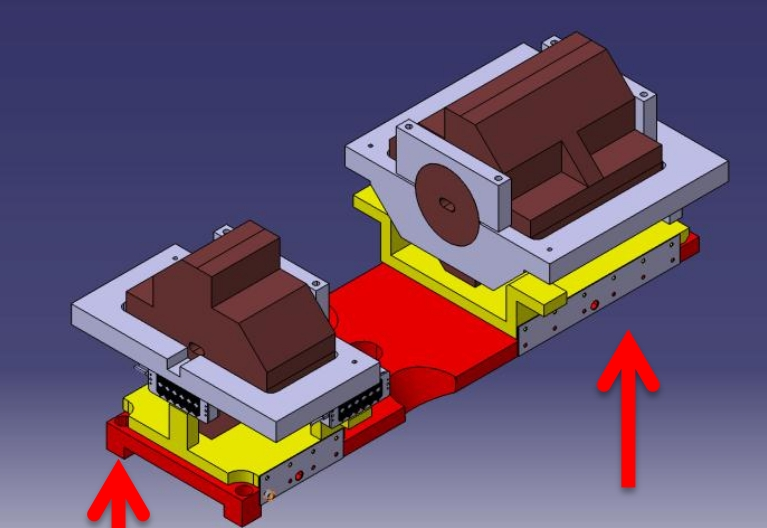
\includegraphics[angle=0,scale=0.22]{BPMs01.jpg}\hspace*{0.2cm}
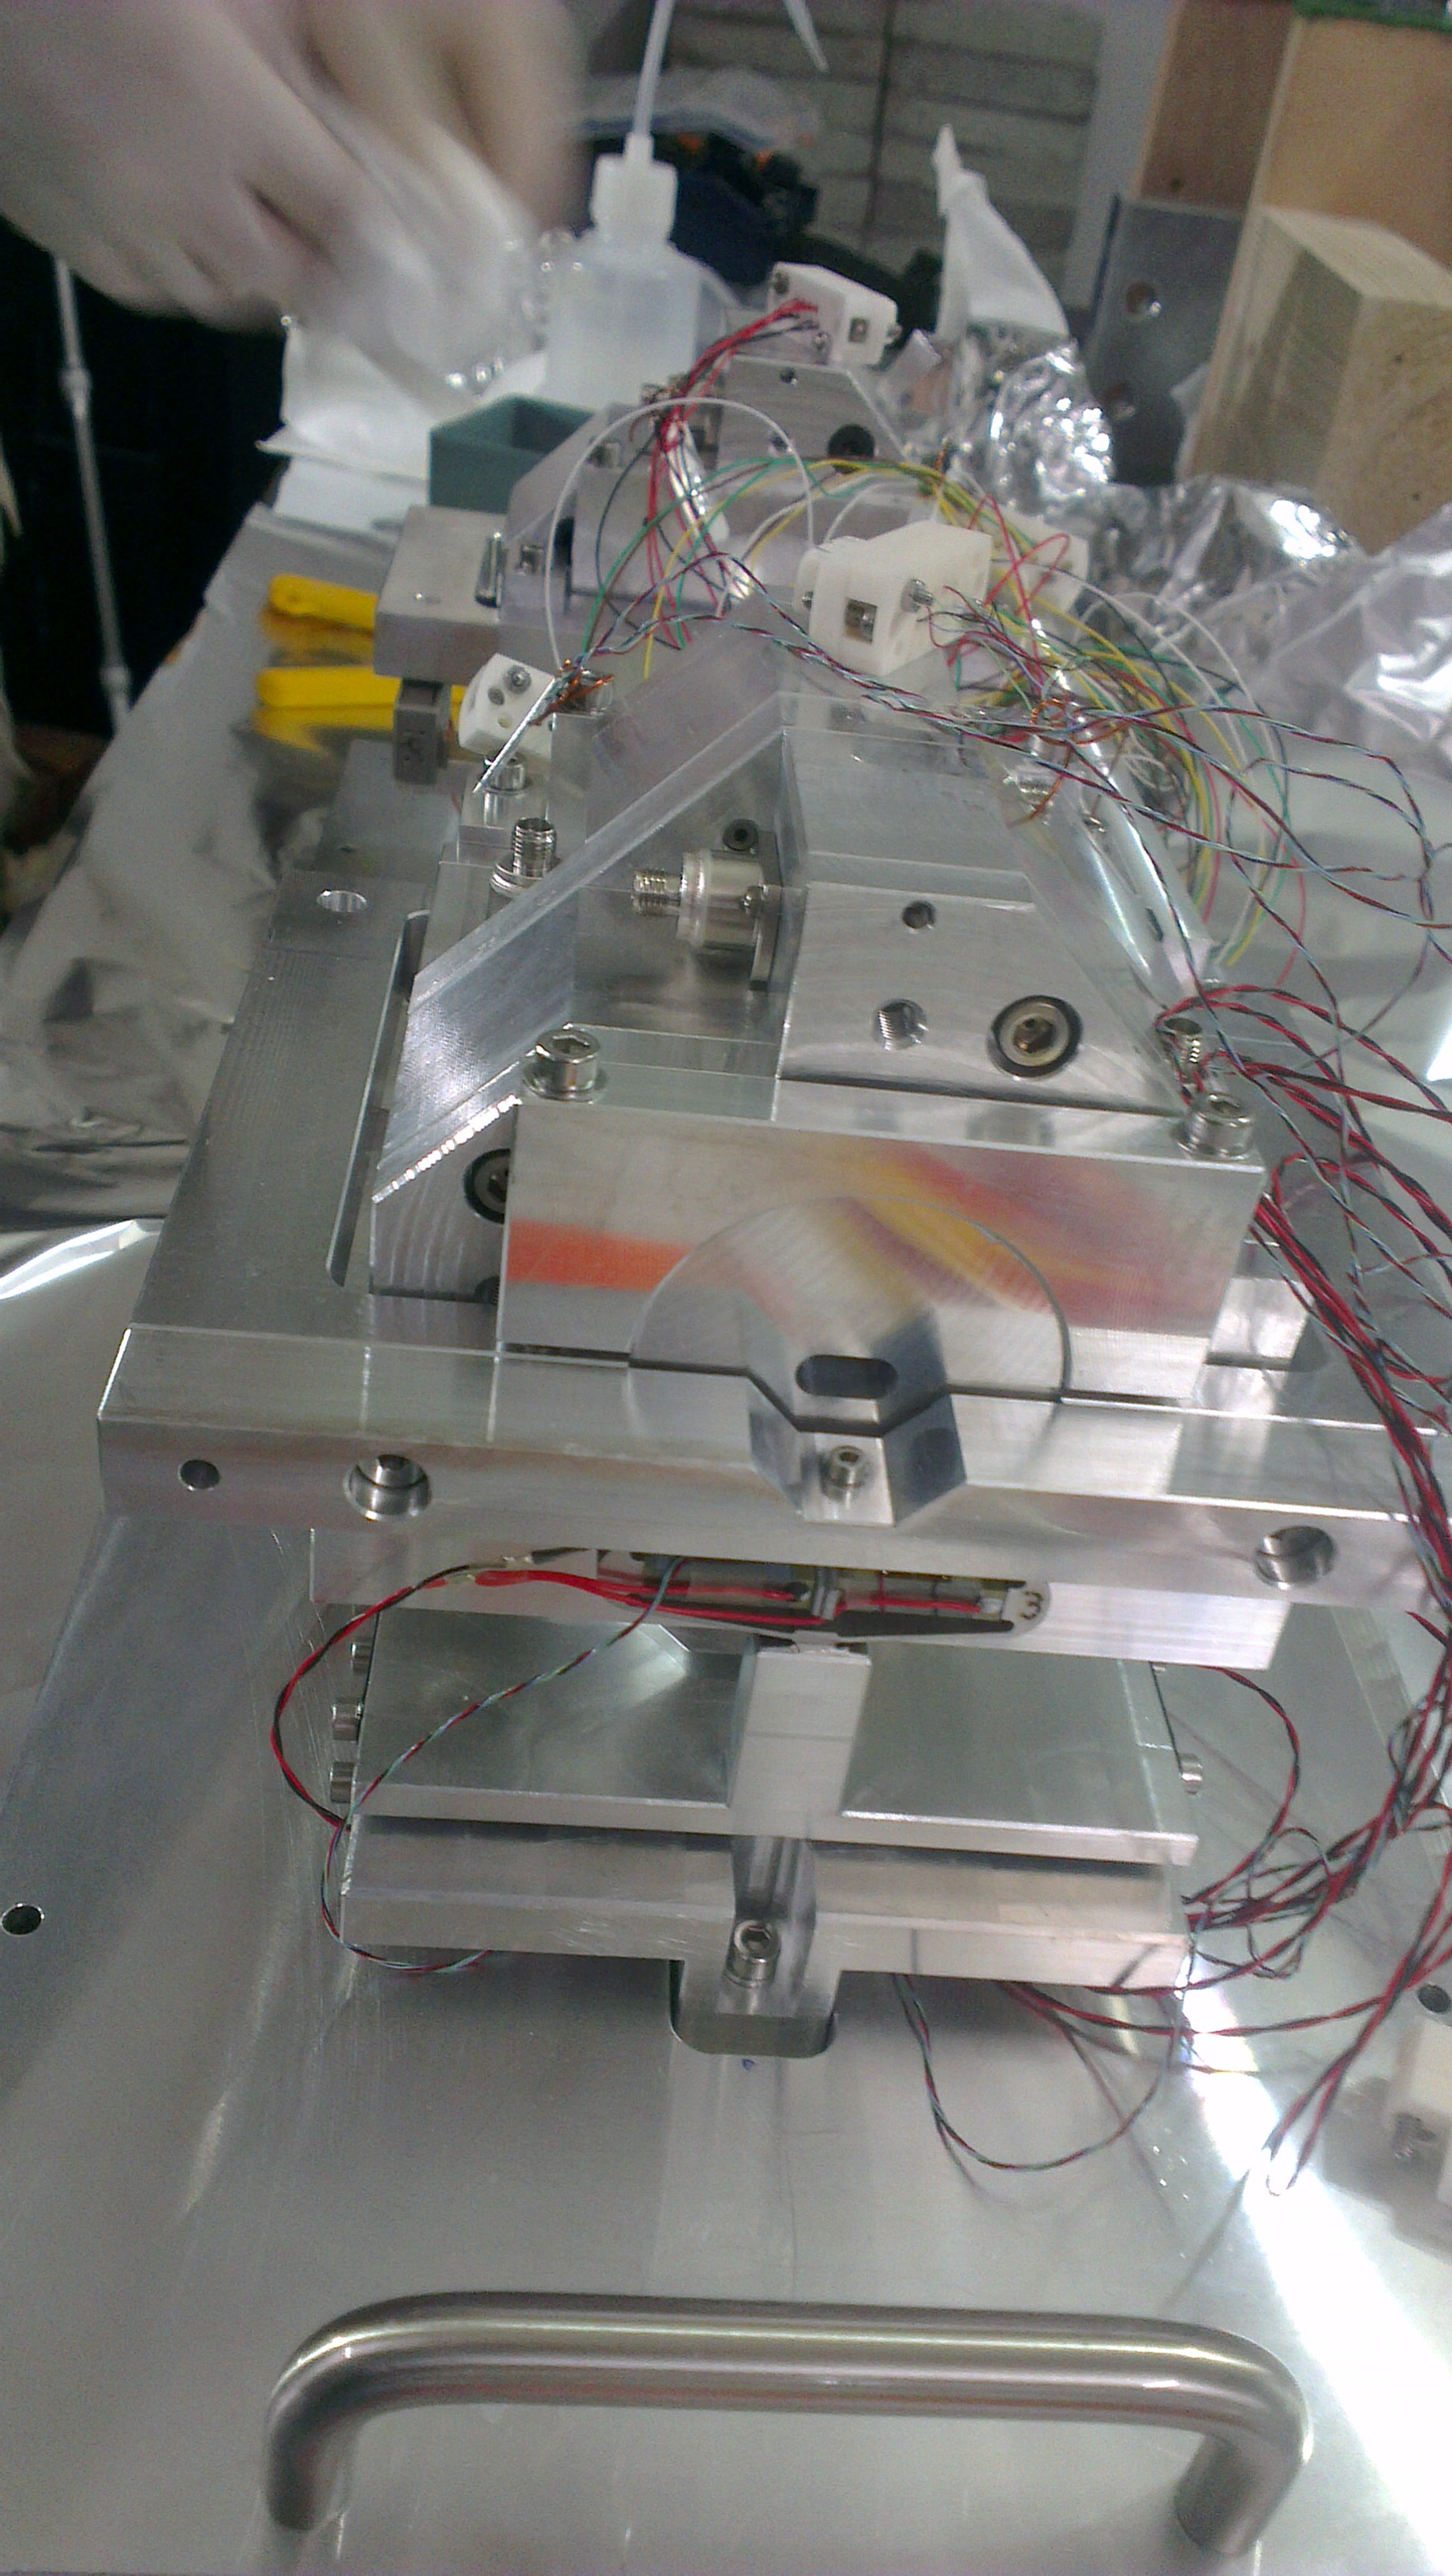
\includegraphics[angle=0,scale=0.0355]{IMAG0460.jpg}\par
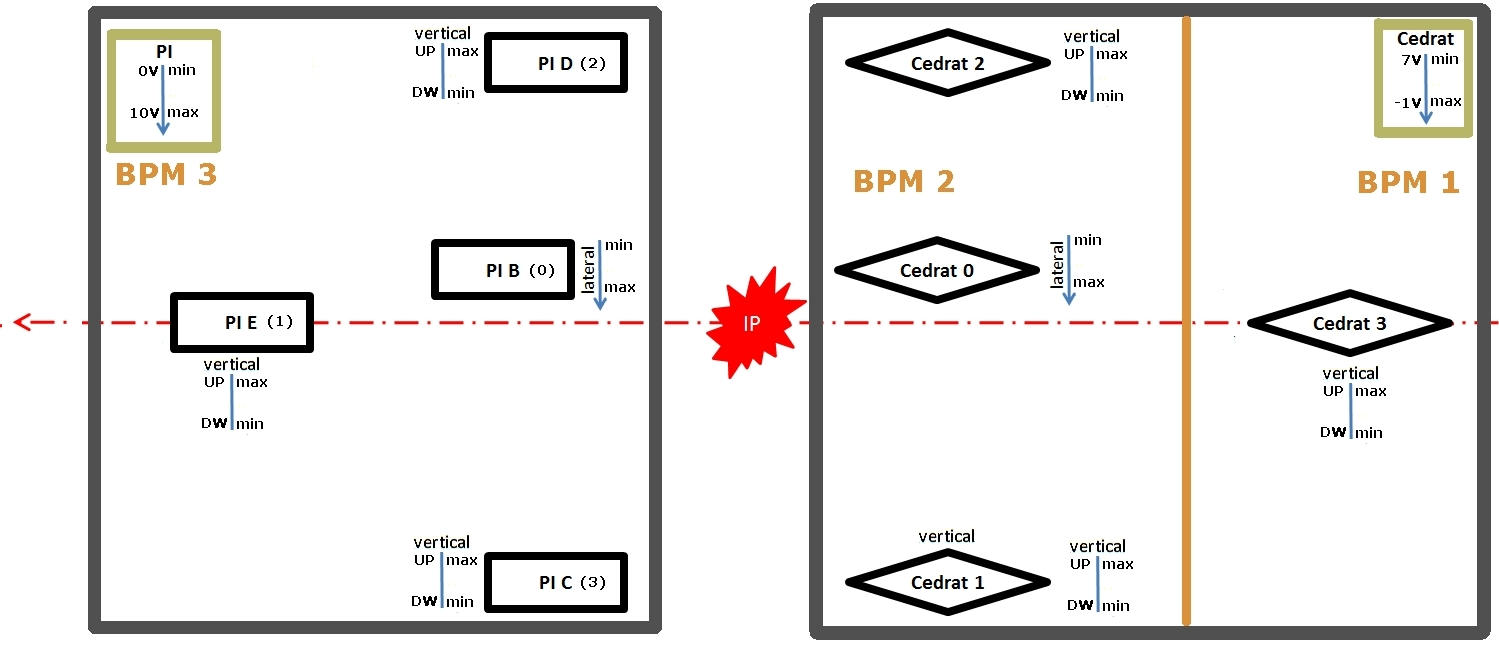
\includegraphics[angle=0,height=7.5cm,width=12cm]{interface.jpg}
